% !TEX TS-program = pdflatex
% !TEX encoding = UTF-8 Unicode

\documentclass[a4paper, titlepage=false, parskip=full-, 10pt]{scrartcl}

\usepackage[utf8]{inputenc}
\usepackage[T1]{fontenc}
\usepackage[english, ngerman]{babel}
\usepackage{babelbib}
\usepackage{hyperref}
\usepackage{listings}
\usepackage{framed}
\usepackage{color}
\usepackage{graphicx}
\usepackage[normalem]{ulem}
\usepackage{cancel}
\usepackage{array}
\usepackage{amsmath}
\usepackage{amssymb}
\usepackage{amsthm}
\usepackage{algorithm}
\usepackage{algorithmic}
\usepackage{geometry}
\usepackage{subfigure}
\geometry{a4paper, top=20mm, left=35mm, right=25mm, bottom=40mm}

\newcounter{tasknbr}
\setcounter{tasknbr}{1}
\newenvironment{task}[1]{{\bf Aufgabe \arabic {tasknbr}\stepcounter{tasknbr}} (#1):\begin{enumerate}}{\end{enumerate}}
\newcommand{\subtask}[1]{\item[#1)]}

% Listings -----------------------------------------------------------------------------
\definecolor{red}{rgb}{.8,.1,.2}
\definecolor{blue}{rgb}{.2,.3,.7}
\definecolor{lightyellow}{rgb}{1.,1.,.97}
\definecolor{gray}{rgb}{.7,.7,.7}
\definecolor{darkgreen}{rgb}{0,.5,.1}
\definecolor{darkyellow}{rgb}{1.,.7,.3}
\lstloadlanguages{C++,[Objective]C,Java}
\lstset{
escapeinside={§§}{§§},
basicstyle=\ttfamily\footnotesize\mdseries,
columns=fullflexible,
keywordstyle=\bfseries\color{blue},
commentstyle=\color{darkgreen},      
stringstyle=\color{red},
numbers=left,
numberstyle=\ttfamily\scriptsize\color{gray},
breaklines=true,
showstringspaces=false,
tabsize=4,
captionpos=b,
float=htb,
frame=tb,
frameshape={RYR}{y}{y}{RYR},
rulecolor=\color{black},
xleftmargin=15pt,
xrightmargin=4pt,
aboveskip=\bigskipamount,
belowskip=\bigskipamount,
backgroundcolor=\color{lightyellow},
extendedchars=true,
belowcaptionskip=15pt}

%% Enter current values here: %%
\newcommand{\lecture}{Robotik WS15/16}
\newcommand{\tutor}{}
\newcommand{\assignmentnbr}{8}
\newcommand{\students}{Julius Auer, Thomas Tegethoff}
%%-------------------------------------%%

\begin{document}  
{\small \textsl{\lecture \hfill \tutor}}
\hrule
\begin{center}
\textbf{Übungsblatt \assignmentnbr}\\
[\bigskipamount]
{\small \students}
\end{center}
\hrule

\begin{task}{A*-Suche}
\item[]
Seien $v$ der Knotenname, $c$ die tatsächlichen Kosten zu einem Knoten, $p$ der Vorgänger auf dem bisher besten Weg und $s\in\{N,O,C\}$ die Zustände der Knoten ($NEW$, $OPEN$ oder $CLOSED$). Dann läuft $A*$ wie folgt:

\begin{minipage}{0.4\textwidth}
\begin{tabular}[!htpb]{r|rrrrrrrr}
$v$&$a$&$b$&$c$&$d$&$e$&$f$&$g$&$h$\\\hline
$c$&$\infty$&$\infty$&$\infty$&$\infty$&$\infty$&$\infty$&$\infty$&$0$\\
$p$&&&&&&&&\\
$s$&N&N&N&N&N&N&N&O
\end{tabular}
\end{minipage}
\hfill
\begin{minipage}{0.4\textwidth}
$OPEN:$\\
$h(19)$
\end{minipage}

$$\Downarrow$$
\begin{minipage}{0.4\textwidth}
\begin{tabular}[!htpb]{r|rrrrrrrr}
$v$&$a$&$b$&$c$&$d$&$e$&$f$&$g$&$h$\\\hline
$c$&$\infty$&$\infty$&$10$&$10$&$10$&$\infty$&$10$&$0$\\
$p$&&&h&h&h&&h&\\
$s$&N&N&O&O&O&N&O&C
\end{tabular}
\end{minipage}
\hfill
\begin{minipage}{0.4\textwidth}
$OPEN:$\\
$g(11), e(30), d(45), c(52)$
\end{minipage}

$$\Downarrow$$
\begin{minipage}{0.4\textwidth}
\begin{tabular}[!htpb]{r|rrrrrrrr}
$v$&$a$&$b$&$c$&$d$&$e$&$f$&$g$&$h$\\\hline
$c$&$\infty$&$\infty$&$10$&$10$&$10$&$20$&$10$&$0$\\
$p$&&&h&h&h&g&h&\\
$s$&N&N&O&O&O&O&C&C
\end{tabular}
\end{minipage}
\hfill
\begin{minipage}{0.4\textwidth}
$OPEN:$\\
$e(30), f(38), d(45), c(52)$
\end{minipage}

$$\Downarrow$$
\begin{minipage}{0.4\textwidth}
\begin{tabular}[!htpb]{r|rrrrrrrr}
$v$&$a$&$b$&$c$&$d$&$e$&$f$&$g$&$h$\\\hline
$c$&$\infty$&$\infty$&$10$&$10$&$10$&$20$&$10$&$0$\\
$p$&&&h&h&h&g&h&\\
$s$&N&N&O&O&C&O&C&C
\end{tabular}
\end{minipage}
\hfill
\begin{minipage}{0.4\textwidth}
$OPEN:$\\
$f(38), d(45), c(52)$
\end{minipage}

$$\Downarrow$$
\begin{minipage}{0.4\textwidth}
\begin{tabular}[!htpb]{r|rrrrrrrr}
$v$&$a$&$b$&$c$&$d$&$e$&$f$&$g$&$h$\\\hline
$c$&$\infty$&$30$&$10$&$10$&$10$&$20$&$10$&$0$\\
$p$&&f&h&h&h&g&h&\\
$s$&N&O&O&O&C&C&C&C
\end{tabular}
\end{minipage}
\hfill
\begin{minipage}{0.4\textwidth}
$OPEN:$\\
$b(39), d(45), c(52)$
\end{minipage}

$$\Downarrow$$
\begin{minipage}{0.4\textwidth}
\begin{tabular}[!htpb]{r|rrrrrrrr}
$v$&$a$&$b$&$c$&$d$&$e$&$f$&$g$&$h$\\\hline
$c$&$40$&$30$&$10$&$10$&$10$&$20$&$10$&$0$\\
$p$&b&f&h&h&h&g&h&\\
$s$&O&C&O&O&C&C&C&C
\end{tabular}
\end{minipage}
\hfill
\begin{minipage}{0.4\textwidth}
$OPEN:$\\
$a(40), d(45), c(52)$
\end{minipage}

$a$ ist gefunden $\rightarrow A*$ terminiert. Gefundener Pfad:
$$h\rightarrow g\rightarrow f\rightarrow b\rightarrow a$$ 
\end{task}

\newpage
\begin{task}{A*-Suche in ROS}
\item[]
Wir bleiben in C++ (falls Wiederverwendung in ROS erforderlich), visualisieren ohne Notwendigkeit aber natürlich nicht in ROS (Bilder mit opencv).

Natürlich ist die Variante implementiert, die Kreise ausschließt. Anstatt eine Liste (mit teuren Operationen) zu verwalten, arbeitet der Algo aber auf einem 2D-Array in dem der \emph{CLOSED}-Status als Zustand für jede Zelle gehalten werden kann (wie auch in Aufgabe 1 gezeigt). Die \emph{OPEN}-Priority-Queue enthält Zeiger  auf diese Zellen. Ansonsten ist A* konventionell implementiert.

Abbildung \ref{fig:2} zeigt die Ergebnisse. Auf den Bildern zeigt die y-Achse nach ''unten'', rote Zellen sind \emph{CLOSED}, graue sind \emph{OPEN}, blaue kennzeichnen das Hindernis, grüne Start- und Zielpunkt und die gelbe Linie den gefundenen Pfad. 

\begin{figure}[!htpb]
\centering
\subfigure[$i=-1$]{
  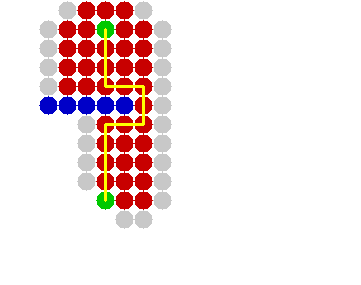
\includegraphics[width=0.48\linewidth]{../../src/u08/captures/capture_2-1}
}
\subfigure[i=0]{
  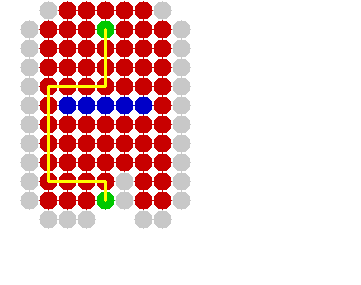
\includegraphics[width=0.48\linewidth]{../../src/u08/captures/capture_2-2}
}
\subfigure[i=1]{
  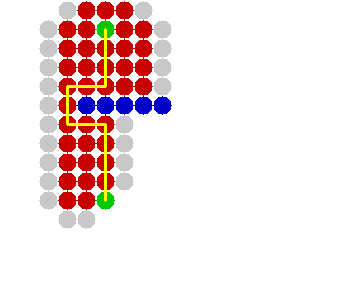
\includegraphics[width=0.48\linewidth]{../../src/u08/captures/capture_2-3}
}
\caption{A*}
\label{fig:2}
\end{figure}
\end{task}
\end{document}